\documentclass[11pt]{article}

\usepackage{titlesec}
\usepackage{graphicx}
\usepackage{caption}
\usepackage{subcaption}
\usepackage{amsmath}
\usepackage{amsfonts}
\usepackage{amssymb}
\usepackage{hyperref}
\usepackage{enumitem}
\usepackage{listings}
\usepackage{xcolor}

% Define colors for syntax highlighting
\definecolor{mygreen}{rgb}{0,0.6,0}
\definecolor{mygray}{rgb}{0.5,0.5,0.5}
\definecolor{mymauve}{rgb}{0.58,0,0.82}

% Set up the MATLAB code listing style
\lstset{
  backgroundcolor=\color{white},
  basicstyle=\footnotesize\ttfamily,
  breakatwhitespace=false,
  breaklines=true,
  captionpos=b,
  commentstyle=\color{mygreen},
  deletekeywords={...},
  escapeinside={\%*}{*)},
  extendedchars=true,
  frame=single,
  keepspaces=true,
  keywordstyle=\color{blue},
  language=Matlab,
  otherkeywords={*,...},
  numbers=left,
  numbersep=5pt,
  numberstyle=\tiny\color{mygray},
  rulecolor=\color{black},
  showspaces=false,
  showstringspaces=false,
  showtabs=false,
  stepnumber=1,
  stringstyle=\color{mymauve},
  tabsize=2,
  title=\lstname
}


% Adjust the margins if needed
\usepackage[left=1in, right=1in, top=1in, bottom=1in]{geometry}
\usepackage{graphicx}
\usepackage{graphicx}
\usepackage{tabto}

% Set the title and author
\title{Solving Systems of Equations, Errors and Explorations}
\author{David Tran and Spencer Kelly}
\date{\today}

\begin{document}

\maketitle

\subsection*{Abstract}
This lab is the 3rd in a series of 4 labs exploring various numerical methods, implementing them, and examining their tradeoffs. In this lab, we explore the PA = LU factorization method for solving systems of linear equations, as well as the Jacobi fixed-point iteration method and multivariate Newton's method. We compare the convergence of the Jacobi FPI and the PA = LU factorization method, and we compare the convergence of Newton's method for different systems of equations. We find that the Jacobi FPI is a simple and easy-to-implement method for solving systems of linear equations, but it is not the most efficient method. We also find that the PA = LU factorization method is not suited for solving systems of linear equations when the matrix is large, and that the Jacobi FPI is much faster and more reliable for this problem. We also find that Newton's method is a very fast and reliable method for solving systems of equations, and that plotting the convergence of Newton's method allows one to understand the rate of convergence and the behavior of the system of equations.

\section{Introduction}

(The citations for the following are found in the references section at the end of the document.)

The problem of solving systems of linear equations forms the historical roots of linear algebra. It was deeply explored by Rene Descartes, who introduced the geometrical interpretation of solutions to systems as intersections in hyper-dimensional Cartesian space. Later, both Leibniz and Gauss independently developed methods for solving systems of linear equations, with the latter being the namesake for Gaussian elimination. 

The methods explored in this lab, namely, PA = LU factorization, Jacobi fixed-point iteration, and Newton's method, are all later methods for solving systems of linear equations. The PA = LU factorization method is a direct substitution method, which means that it is a method that directly computes the solution to the system of linear equations. The Jacobi fixed-point iteration and Newton's method are iterative methods, which means that they are methods that use an initial guess to iteratively compute the solution to the system of linear equations. Both have their tradeoffs, and we will explore these tradeoffs in this lab. We will see why Newton's method is one of the more popular methods for solving systems of equations in modern times.

\section{The PA = LU factorization method for linear systems}

\subsection{Why is PA = LU needed for solving linear systems approximately?}

When solving linear systems of the form $Ax = b$, we begin by gaussian elimination of the matrix $A$, followed by back substitution, and ultimately arrive at our solution.
However, when a particular matrix $A$ is being used for multiple iterations, the overhead involved can become quite an obstacle.
This is because the process of Gaussian elimination is a computationally expensive process, with complexity on the order $O(n^3)$.
But with $PA = LU$ factorization, we essentially remove the overhead involved with Gaussian elimination, for all but the first iteration, by rewriting the matrix $A$ in terms of the upper and lower matrices $L$, and $U$, respectively.
Thus, for every subsequent iteration involving the same matrix, we need not perform gaussian elimination, since $L$ and $U$ allow us to immediately begin performing the second step of solving;
back-substitution, which only has complexity $O(n^2)$.

However, when performing naive Gaussian elimination to form the matrices $L$ and $U$, we are at risk of swamping, or the existence of a zero-pivot.
With the help of a permutation matrix $P$, we can now swap rows and columns, to mitigate the propogation of errors due to multiplying rows by large values, and avoid zero-pivots.
The permutation matrix $P$ keeps track of the swapping of rows and columns, so that the linear system itself remains unperturbed (however it is now written $PAx = Pb$).

A great example would be the system $Ax = b$  with $A = \begin{pmatrix}1 & 2 & 4\\3 & 8 & 14\\ 2 & 6 & 13\\
\end{pmatrix}$.
To begin, we swap rows 1 and 2, since we want our multiplication to be by the smallest values possible during Gaussian elimination.
When doing this, we update our permutation matrix: $P = \begin{pmatrix}0&1&0\\1&0&0\\0&0&1
\end{pmatrix}$, and we can subsequently perform gaussian elimination to yield the matrix $\begin{pmatrix}3&8&14\\(\frac{1}{3})&\frac{-2}{3}&\frac{-2}{3}\\(\frac{2}{3})&\frac{2}{3}&\frac{11}{3}
\end{pmatrix}$, where the brackets around the values in the place of what should be $0$ represents the multiplier for the elimination of the row, (important for bookkeeping when doing permutations).

Once again performing Gaussian elimination we obtain the matrix $\begin{pmatrix}3&8&14\\(\frac{1}{3})&\frac{-2}{3}&\frac{-2}{3}\\(\frac{2}{3})&(-1)&3
\end{pmatrix}$.
From this matrix, we can easily find that $L = \begin{pmatrix}1&0&0\\\frac{1}{3}&1&0\\\frac{2}{3}&-1&1
\end{pmatrix}$ and $U = \begin{pmatrix}3&8&14\\0&\frac{-2}{3}&\frac{-2}{3}\\0&0&3
\end{pmatrix}$.
We can then use these to solve linear systems for $b_k$, with the increased efficiency of $LU$ factorization, and the error mitigation of the pivots enabled by the inclusion of the permutation matrix.\\


\subsection{How to identify systems Ax = b for which PA = LU is not suited}
Although it is a very effective direct method of giving (theoretically) the exact solution of the linear system, PA = LU factorization is not always the tool you want to employ for solving said linear system.
For example, if the matrix involved is positive definite, and symmetric, we can employ methods such as Cholensky Factorization, which is more efficient.
If the matrix is not only positive definite and symmetric, but also sparse, we can employ the Conjugate Gradient Method, which is even more efficient than the aforementioned method, and has even lower memory demand.

\subsection{Larger applications of PA = LU factorization}
The applications of $PA = LU$ factorization extend beyong just solving linear systems,and can be used to solve very common problems.
One such problem is solving for the inverse of a matrix, which is made significantly easier when said matrix is decomposed into upper and lower matrices via $PA = LU$ factorization.
On top of this, we can easily compute the determinant of a matrix given its $PA = LU$ factorization, when we recall that the determinant of a triangular matrix is just its diagonal entries, and that the determinant of a permutation matrix is just $(-1)^n$, where $n$ is the number of rows swapped by the permutation.

\section{Iterative solution of systems of linear equations}

Jacobi FPI is a method for solving systems of linear equations of the form $Ax = b$. It is a multi-dimensional analogue of the one-dimensional fixed-point iteration we explored in Lab 2. We require that $A$ is diagonally dominant, which means that the absolute value of the diagonal element of $A$ is greater than the sum of the absolute values of the other elements in the row. This is a sufficient condition for the convergence of the Jacobi FPI. The Jacobi FPI is given by the following formula:

\begin{equation}
x^{(k+1)} = D^{-1}(L+U)x^{(k)} + D^{-1}b
\end{equation}

where $D$ is the diagonal of $A$, $L$ is the lower triangular part of $A$, and $U$ is the upper triangular part of $A$. The Jacobi FPI is a simple and easy-to-implement method for solving systems of linear equations, but it is not the most efficient method. We will explore the convergence of the Jacobi FPI and compare it to the PA = LU factorization method.

\subsection{Solving an equation for n = 100,000}

We solve the following system of linear equations

\begin{equation}
\begin{bmatrix}
  3 & -1 & 0 & 0 & 0 & \frac{1}{2} \\
  -1 & 3 & -1 & 0 & \frac{1}{2} & 0 \\
  0 & -1 & 3 & -1 & 0 & 0 \\
  0 & 0 & -1 & 3 & 0 & 0 \\
  0 & \frac{1}{2} & 0 & 0 & 3 & -1 \\
  \frac{1}{2} & 0 & 0 & 0 & -1 & 3 \\
\end{bmatrix}x = b
\end{equation}

where $b = (5/2, 3/2, \dots, 3/2, 1, 1, 3/2, \dots, 5/2)^T$, where there are $n - 4$ 3/2's in the middle of the vector. Using the code in Listing \ref{lst:jacobi}, we solve the system of linear equations for $n = 100,000$, with the following:

\begin{verbatim}
>> n = 100000;
>> [A, b] = sparsesetup(n);
>> x = jacobi(A, b, 50);
\end{verbatim}

which converges to $(1, \dots, 1)^T$ after just 50 iterations.



% include code from jacobi.m with a reference
\lstinputlisting[caption={The code for the Jacobi FPI}, label={lst:jacobi}]{jacobi.m}

\subsection{Comparison of PA = LU and Jacobi Iteration}

Theoretically, Jacobi is guaranteed to converge for all $n$ if $A$ is diagonally dominant, which $A$ is in this case. If we try $PA = LU$ decomposition for this problem, using

% include code from solve_lu.m
\lstinputlisting[caption={The code for the LU decomposition}, label={lst:lu}]{solve_lu.m}

the function takes much longer due to its $O(n^3)$ time complexity. Even for $n = 10000$, the function takes almost a minute on an Apple M1 Pro chip. Usually for $PA = LU$, if the matrix is rank-deficient (multiple rows/columns that are linearly dependent), the $LU$ decomposition may not be unique and thus may fail to find the correct solution. However in this case, $A$ is not rank-deficient, so the $LU$ decomposition should work. But, the Jacobi method is much faster and more reliable for this problem.

\subsection{Why is solving such large systems important in applications?}

Solving large systems of linear equations is important in applications because it is a fundamental problem in many areas of science and engineering. For example, in statstics, a linear model may depend on millions or even billions of parameters which translates to a system of equations of the same size. As a concrete example, a dimensonality-reduction technique such as principal component analysis requires solving a system with as many equations as there are data points and/or desired dimensions. Or, for example, modelling fluid dynamics similarily requires very large systems of equations due to the complexity of the problem. Data is naturally highly multi-dimensional, which makes solving large systems important in practice.

\section{Implement Newton's method for multiple variables}


\subsection{Implementation of Newton's method for systems using vectorization}

\lstinputlisting[caption={The code for the Newton's method}, label={lst:newton}]{vectornewton.m}

\subsection{Testing}

We test Newton's method on the following system of equations in Listing \ref{lst:newtontest}: which yields the approximate solution of $u = 1.0960, v = -1.1592, w = -0.2611$ in 7 iterations with a tolerance of $10^{-12}$.
\begin{equation}
\begin{aligned}
  2u^2 - 4u + v^2 + 3w^2 + 6w + 2 &= 0 \\
  u^2 + v^2 - 2v + 2w^2 - 5 &= 0 \\
  3u^2 - 12u + v^2 + 3w^2 + 8 &= 0 \\
\end{aligned}
\end{equation}
In the same code, we solve
\begin{equation}
\begin{aligned}
  y^2 - x^3 &= 0 \\
  x^2 + y^2 - 1 &= 0 
\end{aligned}
\end{equation}
which yields $x = 0.8260, y = 0.5636$ in 7 iterations with a tolerance of $10^{-12}$.


\subsection{Adding Visualization to Newton's Method}

Plotting the convergence of Newton's method allows one to understand the rate of convergence and the behavior of the system of equations, since we often don't know how the system may converge or behave beforehand. For example, We can plot the convergence of Newton's method for the system of equations in Listing \ref{lst:newtontest} by using the code in Listing \ref{lst:vectornewtonvisualized}, which yields the plot in Figure \ref{fig:newtonplot}. It shows that although we don't reach the desired tolerance until iteration 7, the rate of convergence is very fast, and the solution is very close to the true solution after just 4 iterations.

\section{Summary}

\subsection{Results}

We explored 3 different methods of solving systems of equations across 2 different categories: direct substitution methods, and iterative methods. We found that the Jacobi FPI is a simple and easy-to-implement method for solving systems of linear equations, but it is not the most efficient method. We also found that the PA = LU factorization method is not suited for solving systems of linear equations when the matrix is large, and that the Jacobi FPI is much faster and more reliable for this problem. We also implemented Newton's method for systems of equations and found that it is a very fast and reliable method for solving systems of equations, and that plotting the convergence of Newton's method allows one to understand the rate of convergence and the behavior of the system of equations.

\subsection{Team Work Problems and Ideas}

We worked well together and were able to complete the lab in a timely manner. We were able to divide the work evenly and work on the lab together. We were able to communicate effectively and work together to solve the problems in the lab. A problem that was encountered was in the testing of the PA = LU method, where the function took much longer than expected to run. We were able to solve this problem by starting with much smaller input sizes (e.g. $n = 100$) and growing $n$ much slower to see how the function scaled.
\subsection{Future Explorations}

In the future, we would like to explore other methods for solving systems of equations, such as the Gauss-Seidel method, the SOR method, and the conjugate gradient method. We would also like to explore the convergence of these methods and compare them to the methods we explored in this lab. We would also like to further explore how ill-conditioned matrices may behave with the discussed methods, and how to transform the matrices to be better conditioned.

\begin{thebibliography}{}
  \bibitem{christensen2012}
  Christensen, R. H. (2012).
  \textit{The History of Linear Algebra}.
  Retrieved from: \url{https://www.math.utah.edu/~gustafso/s2012/2270/web-projects/christensen-HistoryLinearAlgebra.pdf}
  
  \bibitem{fearnley1979}
  Fearnley-Sander, D. (1979).
  \textit{Hermann Grassmann and the Creation of Linear Algebra}.
  \textit{American Mathematical Monthly}, 86, 809–817.
  
  \bibitem{hart2010}
  Hart, R. (2010).
  \textit{The Chinese Roots of Linear Algebra}.
  JHU Press. ISBN 9780801899584.
  
  \bibitem{sauer2012}
  Sauer, T. (2012).
  \textit{Numerical Analysis}.
  Pearson. ISBN 978-0-321-58746-2.
\end{thebibliography}
  

\section{Appendices}

\subsection{Code}

\lstinputlisting[caption={The code for the Newton's method test}, label={lst:newtontest}]{vectornewtontest.m}

\lstinputlisting[caption={The code for the Newton's method with visualization}, label={lst:vectornewtonvisualized}]{vectornewtonvisualized.m}

\subsection{Plots}

\begin{figure}[h]
  \centering
  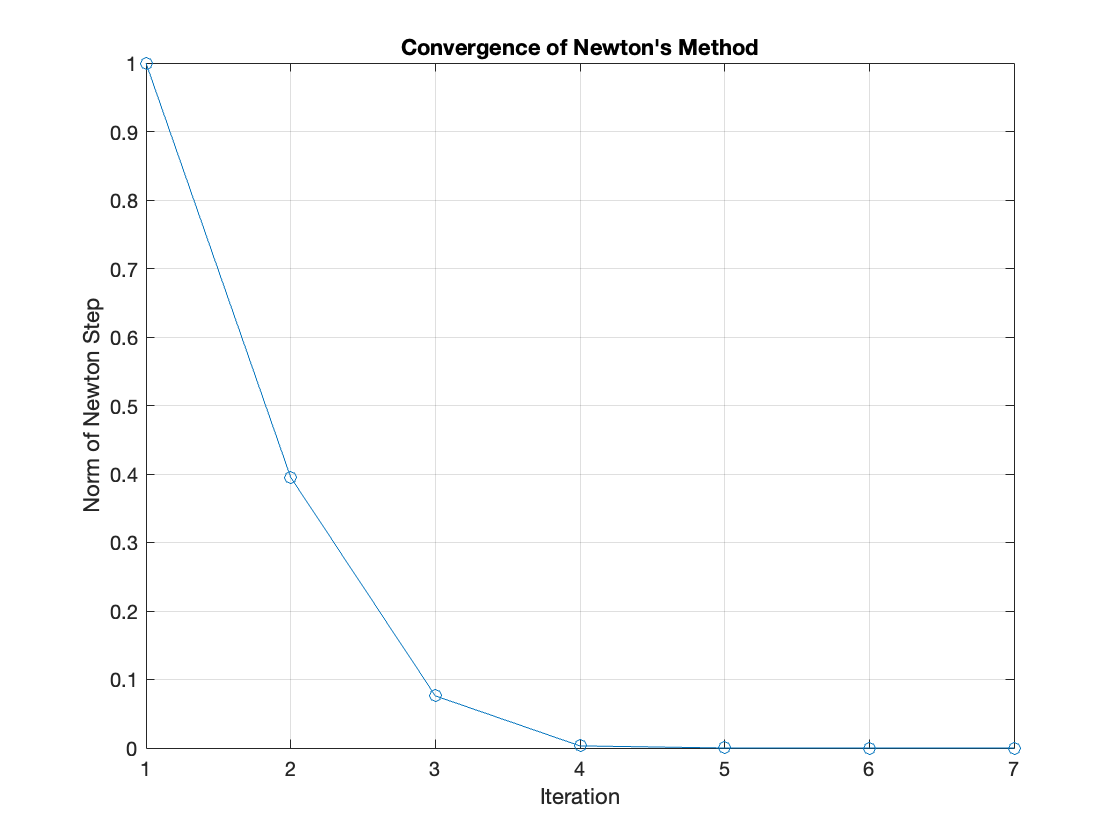
\includegraphics[width=\textwidth]{newtonplot.png}
  \caption{The convergence of Newton's method for the second system of equations in Listing \ref{lst:newtontest}}
  \label{fig:newtonplot}
\end{figure}


\end{document}
